\chapter{Architektura II: uwaga, kontekst i głowice}\label{rozdz:uwaga-wys}

\section{Co jeszcze potrafi poprawić wektor opisu?}

Po pierwszej połowie sieci każda para (klatka $t$, półton $s$) ma wektor $h_{t,s}\in\R^{64}$ opisujący, ile jest tam „śladów nuty” (rozdział~\ref{rozdz:architektura}). Brakuje dwóch rzeczy.
Po pierwsze \emph{czasu}: czy nuta trwa od poprzedniej klatki, czy to nowe szarpnięcie, czy koniec? Po drugie \emph{sąsiedztwa}: jeśli oktawę niżej też coś gra, czy to naprawdę osobna nuta, czy tylko alikwot? Obie rzeczy załatwia uwaga (rozdział~\ref{rozdz:uwaga}):
raz wzdłuż osi czasu, raz wzdłuż osi wysokości.

Po tym rozdziale umiesz: (i)~zapisać jedną warstwę kontekstu, (ii)~policzyć pole widzenia całej sieci i porównać je z pomiarem, (iii)~wyjaśnić działanie głowic i głowicy tabulatury, (iv)~policzyć liczbę parametrów całej sieci.

\section{Warstwa kontekstu}

\haslo{warstwa kontekstu}
\begin{definicja}[Warstwa kontekstu]\label{def:ctx}
Wejście $h\in\R^{T\times S\times D}$ ($T$ klatek, $S=53$ półtony, $D=64$). \emph{Warstwa kontekstu} liczy kolejno (zawsze z normalizacją przed funkcją i połączeniem resztkowym, rys.~\ref{rys:blok}):
\begin{align*}
h' &= h+\Drop\big(\mathrm{TA}(\LN(h))\big), \\
h'' &= h'+\Drop\big(\mathrm{PA}(\LN(h'))\big), \\
h''' &= h''+\Drop\big(\mathrm{FF}(\LN(h''))\big),
\end{align*}
gdzie $\mathrm{TA}$ to uwaga w czasie, $\mathrm{PA}$ uwaga między wysokościami, a $\mathrm{FF}(z)=W_2\,\GELU(W_1z)$ z $W_1\colon\R^{64}\to\R^{256}$, $W_2\colon\R^{256}\to\R^{64}$. Sieć ma dwie takie warstwy.
\end{definicja}

\begin{przyklad}\label{prz:ctx-param}
Parametry jednej warstwy: trzy LayerNorm po $2\cdot64=128$ ($384$), $\mathrm{TA}$ ($16\,988$), $\mathrm{PA}$ ($17\,060$) i $\mathrm{FF}$ ($64\cdot256+256+256\cdot64+64=33\,088$), razem $67\,520$. Dwie warstwy mają $135\,040$ parametrów, czyli ponad połowę całej sieci ($249\,219$).
\end{przyklad}

\section{Uwaga w czasie}

Dla każdego półtonu $s$ osobno bierzemy ciąg wektorów $h_{1,s},\dots,h_{T,s}$ i stosujemy uwagę z rozdziału~\ref{rozdz:uwaga} z oknem $\abs{j-i}\le W=43$ klatek ($43\cdot23{,}2\ms\approx1$ s) w obie strony i wyuczoną premią $b^{\mathrm{(czas)}}_{j-i}$ (osobną dla każdej z $n_h=4$ głowic, $87$ wartości):
\begin{equation}
  \alpha^{\mathrm{(czas)}}_{ij}=\softmax_{j:\,\abs{j-i}\le W}\Big(\frac{\ip{\vect q_i}{\vect k_j}}{\sqrt{d_h}}+b^{\mathrm{(czas)}}_{j-i}\Big),\qquad d_h=\frac{D}{n_h}=16.
\end{equation}

\begin{intuicja}
Sieć sprawdza, czy ten sam półton brzmiał w klatkach sprzed i po: jeśli tak, to nuta „trwa”; jeśli ślad zaczyna się nagle i wcześniej go nie było, to początek; jeśli zanika, to koniec. Okno $\pm1$ s wystarcza, by rozstrzygnąć powtórzenie nuty lub jej koniec.
Wariant przyczynowy (tylko $j\le i$) nadaje się do pracy na żywo, ale Gen~6 w tej książce jest używany w trybie dwukierunkowym (analiza całego nagrania).
\end{intuicja}

Okno ma praktyczną zaletę: koszt to $O(T\cdot(2W+1))$ zamiast $O(T^2)$. Implementacja w repozytorium dzieli oś czasu na bloki długości $W$ i pozwala blokowi patrzeć na dwa sąsiednie.

\section{Uwaga między wysokościami}

W jednej klatce $t$ traktujemy $53$ półtony jako sekwencję i stosujemy uwagę \emph{bez okna} ($53\times53$ wag), z premią zależną od odległości w półtonach $r_{j-i}$, $j-i\in\{-52,\dots,52\}$ ($105$ wartości na głowicę):
\begin{equation}
  \alpha^{\mathrm{(wys)}}_{ij}=\softmax_{j}\Big(\frac{\ip{\vect q_i}{\vect k_j}}{\sqrt{d_h}}+r_{j-i}\Big).
\end{equation}
Zadanie tej uwagi jest dokładnie tym, czego brakowało w rozdziale~\ref{rozdz:alikwoty}: pozwolić każdemu półtonowi zerknąć na pozostałe, w szczególności na te leżące o $12$, $19$, $24$ półtonów od niego (interwały alikwotów) oraz na inne nuty akordu.

\begin{naliczbach}
Rozmiary dla klatki: $Q,K,V\in\R^{53\times16}$ dla każdej z $4$ głowic, macierz wag $53\times53=2809$ liczb na głowicę. Jeśli zapytanie jest podobne tylko do własnego klucza i do kluczy odległych o $\pm12$, a premia $r_{\pm12}$ jest duża, to waga skupia się na tych trzech półtonach (zabawkowy przypadek w rozdziale~\ref{rozdz:uwaga}, rys.~\ref{rys:uwaga}a).
\end{naliczbach}

\begin{twierdzenie}[Pole widzenia sieci]\label{tw:pole-sieci}
Niech część konwolucyjna ma pole widzenia w czasie $R_\mathrm{conv}$ (tw.~\ref{tw:pole-widzenia}), a $n_\mathrm{ctx}$ warstw kontekstu używa uwagi z oknem $\abs{j-i}\le W$. Wtedy wynik w klatce $t$ zależy od wejść w klatkach $t'$ z $\abs{t'-t}\le R=R_\mathrm{conv}+n_\mathrm{ctx}W$ i (dla niezerowych wag) tylko od nich.
\end{twierdzenie}
\begin{pomyslDowodu}
Każda warstwa uwagi z oknem $W$ miesza cechy z klatek odległych o najwyżej $W$; kolejne warstwy rozszerzają zasięg tak jak kolejne konwolucje: odległości się dodają.
\end{pomyslDowodu}
\begin{proof}
Indukcja po warstwach, jak w dowodzie tw.~\ref{tw:pole-widzenia}. Po części konwolucyjnej wektor $h_{t,\cdot}$ zależy od wejść $X_{t'}$ z $\abs{t'-t}\le R_\mathrm{conv}$. Uwaga w czasie liczy nowy wektor w klatce $t$ jako średnią ważoną wartości z klatek $u$ z $\abs{u-t}\le W$, a każda z nich zależy od wejść odległych o $\le R_\mathrm{conv}$ od $u$:
\begin{align*}
\abs{t'-t}\le\abs{t'-u}+\abs{u-t}\le R_\mathrm{conv}+W && \pow{(nierówność trójkąta)}
\end{align*}
Uwaga między wysokościami działa w jednej klatce i nie zmienia zasięgu w czasie; FF i LN są punktowe. Po $n_\mathrm{ctx}$ warstwach zasięg to $R_\mathrm{conv}+n_\mathrm{ctx}W$. To kończy dowód.
\end{proof}

Dla Gen~6: $R_\mathrm{conv}=8$ (przykład~\ref{prz:pole-gen6}), $n_\mathrm{ctx}=2$, $W=43$, czyli $R=8+2\cdot43=94$ klatki, czyli $\pm94\cdot23{,}2\ms=\pm2{,}18$ s. \textbf{Pomiar potwierdza}: gradient logitu początku w jednej klatce po wejściu jest niezerowy dokładnie dla $\abs{t'-t}\le94$ i równy zeru od $95$ (rys.~\ref{rys:pole-modelu}).
Gradient maleje szybko z odległością: $37{,}5$ dla $t'=t$, $2{,}6$ dla odległości $40$, $0{,}035$ dla $90$. Model „słucha” więc głównie najbliższych ok.\ $\pm1$ s, a dalszy kontekst ma niewielki wpływ.

Kod repozytorium używa przy wnioskowaniu kawałkami zakładki \texttt{halo}$=1+7+n_\mathrm{ctx}\cdot2W=180$ klatek z każdej strony; to \emph{zapas bezpieczeństwa} prawie dwukrotnie większy niż rzeczywiste $94$ (każdą warstwę policzono jak $2W$ zamiast $W$). Dlatego wynik nie zależy od długości kawałka; sprawdzono to numerycznie (różnica poniżej $10^{-5}$).

\begin{figure*}[ht]
\centering
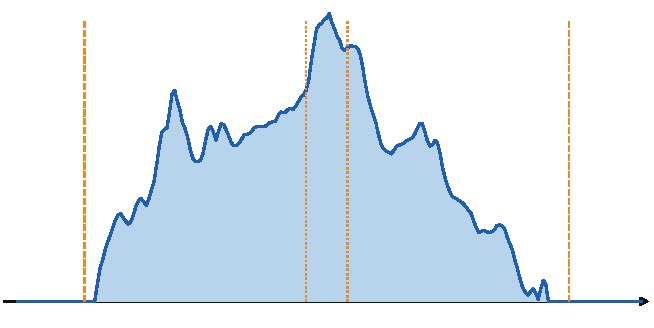
\includegraphics[width=0.62\linewidth]{figures/pole-widzenia-modelu.pdf}
\caption{Pomiar pola widzenia prawdziwego modelu Gen~6: $\log_{10}$ modułu gradientu logitu początku w klatce $t$ (jeden półton) po cechach wejściowych w klatce $t+\Delta t$, od $-125$ do $125$ klatek (pomarańczowe pionowe: kropkowane $\pm8$ --- zasięg samej części konwolucyjnej,
przerywane $\pm94$ --- zasięg całej sieci). Poza $\pm94$ zależności nie ma (wypełnienie opada do dna skali); wewnątrz maleje o kilka rzędów wielkości.}
\label{rys:pole-modelu}
\end{figure*}

\begin{figure*}[ht]
\centering
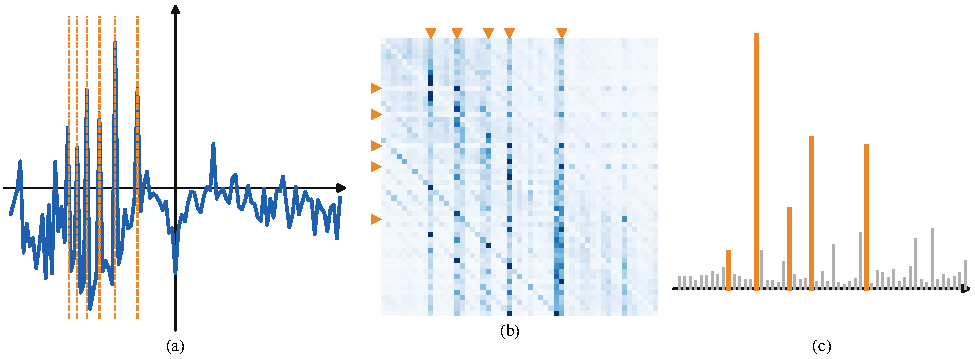
\includegraphics[width=\linewidth]{figures/uwaga-wysokosci.pdf}
\caption{Uwaga między wysokościami w prawdziwym modelu Gen~6 (warstwa kontekstu 0). (a) Wyuczona premia $r_d$ głowicy $2$: niebieska krzywa, pomarańczowe przerywane linie to odległości $-12\log_2h$ dla $h=2,\dots,7$ ($-12,-19,-24,-28,-31,-34$). Dokładnie siedem odległości ma premię powyżej $0{,}6$:
sześć z nich to te interwały alikwotów, a siódma to $+12$. (b) Macierz wag uwagi (średnia z czterech głowic; wiersz --- zapytanie, kolumna --- klucz) w klatce nagrania, w której gra $5$ nut (pomarańczowe znaczniki przy osiach to ich półtony). (c) Wiersz najniższej nuty ($m=45$):
pomarańczowe słupki to pozostałe nuty akordu; trafia w nie $45\%$ całej wagi, podczas gdy równomierny rozkład dałby $4/53=7{,}5\%$.}
\label{rys:uwaga-wys}
\end{figure*}

\subsection{Co się nauczyła uwaga: obserwacja, nie dowód}

Rysunek~\ref{rys:uwaga-wys} pokazuje dwie rzeczy, które sieć odkryła sama, bez żadnej podpowiedzi poza stratą. \textbf{(1)} Jedna z czterech głowic pierwszej warstwy ma największe premie na odległościach równych interwałom szeregu alikwotów ($12,19,24,28,31,34$ półtonów w dół):
dokładnie tym, które w rozdziale~\ref{rozdz:alikwoty} wyliczyliśmy jako $12\log_2h$. Taką głowicę można czytać tak: „kandydat $s$ patrzy na półtony, w których leżałyby jego alikwoty, i sprawdza, czy tam coś jest”. \textbf{(2)} W klatce z akordem uwaga najniższej nuty
koncentruje się na pozostałych nutach akordu. Inne głowice mają premie największe na małych odległościach ($\pm1$ do $\pm5$): sąsiedzi półtonowi.

Uczciwie: to \emph{korelacje w wagach}, nie dowód przyczynowy. Nie badaliśmy, co się stanie, gdy dany interwał lub głowicę usuniemy (brak badań ablacyjnych --- zob.\ rozdział~\ref{rozdz:wyniki}); premie nie mówią, czy dana głowica jest \emph{potrzebna}, tylko czego sieć użyła.

\begin{pulapka}
Zwykła pokusa: zobaczyć na mapie uwagi „ładny wzór” i uznać, że sieć działa zgodnie z naszą teorią. Wagi w jednym nagraniu i jednej klatce to jeden punkt; warto sprawdzić, czy wzór utrzymuje się na wielu nagraniach (tu: premie są własnością wag, więc nie zależą od nagrania, a mapa (b) tak).
\end{pulapka}

\section{Głowice}

Po dwóch warstwach kontekstu i LayerNorm mamy $h_{t,s}\in\R^{64}$. Każda głowica to małe MLP, $\MLP(z)=W_2\GELU(W_1z)$:
\begin{align*}
p_\mathrm{on} &= \sigma\big(\MLP_\mathrm{on}(h)\big), & p_\mathrm{fr} &= \sigma\big(\MLP_\mathrm{fr}([\,h\,;\ \sg(p_\mathrm{on})\,])\big),\\
p_\mathrm{off} &= \sigma\big(\MLP_\mathrm{off}(h)\big), & \hat v &= \sigma\big(\MLP_\mathrm{vel}(h)\big),
\end{align*}
gdzie $[\,\cdot\,;\cdot\,]$ to sklejenie ($65$ wejść do głowicy „brzmi”), a $\sg(\cdot)$ to \emph{stop-gradient}: głowica „brzmi” dostaje $p_\mathrm{on}$ jako cechę, ale jej strata nie zmienia głowicy początku (pomysł z \emph{Onsets and Frames}).
Obciążenia ostatnich warstw ustawiono na $-3$ (początek, koniec) i $-2$ (brzmi), by zacząć od „nut jest mało” (rozdział~\ref{rozdz:strata}).

\begin{naliczbach}
Głowica początku: $64\cdot64+64+64+1=4225$. Głowica „brzmi” z $65$ wejściami: $65\cdot64+64+65=4289$. Głowice końca i głośności po $4225$. Razem z tabulaturą ($4735$) i końcowym LayerNorm ($128$): $4225+4289+4225+4225+4735+128=21\,827$.
Pełna suma: $92\,352$ (pierwsza połowa) $+\ 135\,040$ (kontekst) $+\ 21\,827=249\,219$ --- dokładnie tyle, ile liczy sieć w repozytorium (sprawdzone programem).
\end{naliczbach}

\haslo{głowica tabulatury}
\begin{definicja}[Głowica tabulatury]\label{def:tab}
Dla struny $i\in\{1,\dots,6\}$ z wysokością struny pustej $o_i$ i progu $f\in\{0,\dots,19\}$ półton $s_{i,f}=o_i+f-36$ (jeśli leży w $[0,52]$; inaczej logit jest $-\infty$). Logit
\begin{equation}
  g_{i,f}(t)=\vect w_i^{\top}h_{t,s_{i,f}}+c_i+\beta_{i,f},
\end{equation}
gdzie $\vect w_i\in\R^{64}$, $c_i$ --- wagi i obciążenie \emph{osobne dla każdej struny}, a $\beta_{i,f}$ --- wyuczona premia za próg (wysokie progi są rzadsze). Klasa „struna $i$ milczy”: $g_{i,\varnothing}(t)=\MLP_\mathrm{sil}\big(\max_f h_{t,s_{i,f}}\big)$ (maksimum po $f$ dla każdego kanału osobno).
Wynik: $p_i=\softmax(g_{i,\varnothing},g_{i,0},\dots,g_{i,19})$, czyli $21$ klas na strunę.
\end{definicja}

\begin{przyklad}\label{prz:tab-b3}
Struna~2 (B3, $o_2=59$): progi $f=0,\dots,19$ odpowiadają półtonom $s=23,\dots,42$ (nuty MIDI $59$--$78$). Logit „struna~2 gra próg $5$” to $\vect w_2^{\top}h_{t,28}+c_2+\beta_{2,5}$, czyli liczy się z cech półtonu $28$ (E4), a nie z cech dla progu. Parametry głowicy: $\vect w_i,c_i$ razem $6\cdot65=390$, premie $\beta$ $6\cdot20=120$, MLP ciszy $64\cdot64+64+64+1=4225$; razem $4735$.
\end{przyklad}

\begin{intuicja}
Logit „struna $i$ gra próg $f$” liczymy z cech tego półtonu, który ten próg produkuje. Dzięki temu tabulatura jest \emph{powiązana} z detekcją wysokości: gdy sieć wie, że gra E4, pozostaje jej rozstrzygnąć, na której z pięciu strun (rozdział~\ref{rozdz:dane}).
Osobne $\vect w_i$ pozwalają każdej strunie mieć własną „barwę” (rozkład alikwotów zależy od grubości struny).
\end{intuicja}

\section*{Podsumowanie}
\begin{itemize}
\item Warstwa kontekstu: uwaga w czasie (okno $\pm43$ klatki), uwaga między wysokościami ($53\times53$) i FF, każda z LN i połączeniem resztkowym; dwie warstwy $=135\,040$ parametrów.
\item Pole widzenia sieci $R=R_\mathrm{conv}+n_\mathrm{ctx}W=8+86=94$ klatki ($\pm2{,}18$ s) --- potwierdzone pomiarem gradientu; kod używa zapasu $180$.
\item Jedna z głowic uwagi między wysokościami ma największe premie na interwałach alikwotów; uwaga najniższej nuty akordu trafia w pozostałe nuty (obserwacja z wag, bez ablacji).
\item Pięć głowic: początek, brzmi (z $\sg(p_\mathrm{on})$), koniec, głośność (nieuczona), tabulatura (softmax po $21$ klasach na strunę).
\item Parametry: $92\,352+135\,040+21\,827=249\,219$.
\end{itemize}

\begin{sprawdz}
\begin{enumerate}
\item Policz pole widzenia $R$, gdyby $n_\mathrm{ctx}=3$, $W=30$ i $R_\mathrm{conv}=8$. Ile to sekund przy kroku $23{,}2\ms$?
\item Ile parametrów miałaby warstwa kontekstu bez uwagi między wysokościami (zostają LN dla TA i FF: dwa LayerNorm)?
\item Wyznacz półtony $s_{i,f}$ dla struny~6 ($o_6=40$) i progów $f=0,12,19$. Ile klas ma głowica tabulatury łącznie dla wszystkich strun?
\item Dla jakich $s_{1,f}$ (struna~1, $o_1=64$) logit jest $-\infty$ w modelu z $S=53$ półtonami i progami $0$--$19$?
\end{enumerate}
\end{sprawdz}

\subsection*{Rozwiązania}
\begin{enumerate}
\item $R=8+3\cdot30=98$ klatek; $98\cdot23{,}2\ms=2{,}27$ s.
\item $2\cdot128+16\,988+33\,088=50\,332$ (zamiast $67\,520$; różnica $17\,188=17\,060+128$).
\item $s_{6,f}=40+f-36$: $4,\,16,\,23$. Klas: $6\cdot21=126$ (liczba wyjść głowicy tabulatury w jednej klatce).
\item $s_{1,f}=64+f-36=28+f$; dla $f=0,\dots,19$ to $28,\dots,47\le52$, więc żaden logit nie jest $-\infty$ dla struny~1 (wszystkie pozycje mieszczą się w zakresie $0$--$52$).
\end{enumerate}
